%====================================================================
\subsection{Parallel implementation}\label{chap:parallel}
%====================================================================




\ramses\ is a parallel code which makes use of the MPI standard.
The use of MPI (message passing interface) allows a process on a distributed memory architecture to be executed in parallel by multiple tasks and defines various types of communications between them.

The fundamental parallelisation strategy used in \ramses\ is domain decomposition,
where a part of the total spatial computational domain is assigned to each processing unit, or ``\emph{MPI task}''.
It makes use of the fact that most calculations on grids do not require the knowledge of the entire computational domain, but only the cells in their vicinity.
The basic idea of the domain decomposition is illustrated in figure \ref{fig:parallel}, where a 2D-grid is split between two processors. 
The partial domains do not overlap and a thin layer of cells, called the ``\emph{virtual boundary}'', is introduced where the domain was cut. 
Only necessary information is then communicated across MPI tasks from the other tasks' ``real domain'' into the virtual boundary, so that the virtual boundary copies what happens in the domains of other tasks, allowing the execution of the code as if the domain wasn't split.
Two tasks working on the same problem allows a much faster execution time, but it also enables the solution of bigger problems that only one task couldn't do on its own, e.g. because of memory restrictions.

\begin{figure}[htbp]
	%\parpic[r]{%
	\centering
	\fbox{
		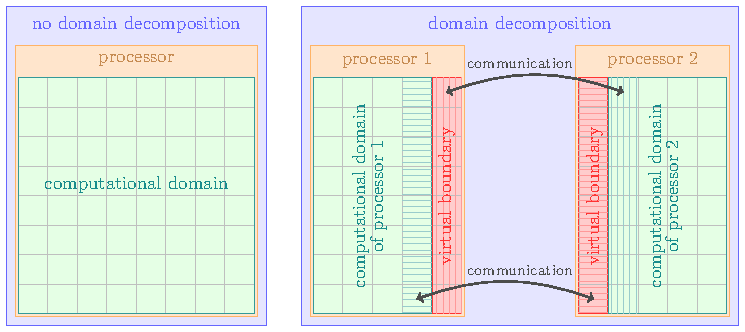
\includegraphics[width = 12.5cm, keepaspectratio]{images/tikz/parallelisation.pdf}
	}
	\caption{
		The basic idea of domain decomposition. Here a 2D-grid is split between two processors (right) instead of only one (left). 
		The partial domains do not overlap and where the domain was cut, a  ``virtual boundary'' is introduced. 
		Necessary information is then communicated between processors from the other tasks' ``real domain'' into the virtual boundary, so that the virtual boundary copies what happens in the domains of other tasks and allows the execution of the code as if the domain wasn't split.
	}
	\label{fig:parallel}
\end{figure}




\phew\ uses the virtual mesh boundary as well, since every cell on each domain must have the information of all its neighbours.
%Initially, all peaks are counted and their number is communicated throughout all MPI tasks.
%This gives all MPI tasks the knowledge of the total number of peaks of the entire computational domain, allowing the introduction of a peak label that is globally unique for each peak. 
Similarly to the virtual mesh boundary, a virtual peak boundary is necessary.
For the peak patch merging step, each peak patch on each task's domain needs the information of the peak patches that surround it.
If, for example, a peak patch is split in two by the domain boundaries between two tasks, both tasks need to know all the peak patch's neighbours on the other task's domain.
%
Unlike the mesh boundary however, the virtual peak boundary is not a fixed region in space.
Because of the merging, peaks gain neighbours they hadn't had before.
This requires that new peaks are introduced to the virtual peak boundary during the merging procedure.
%Virtual peaks are introduced by assigning them a local peak index.
%Each tasks stores the virtual peaks in the first free place in the memory after the ``real'' peaks.
Once introduced, all other peak properties, e.g. its relevance and saddle points, can be transferred by means of MPI communication.

The virtual peak boundary requires two types of communications. 
One type is the collection (sum, minimum or maximum) of a value for a peak from all tasks which have that particular peak patch in their virtual boundary to the owner of the peak.
The ``\emph{owner}'' of the peak is the task where the density peak is in the ``real'' domain, as opposed to the virtual mesh boundary.
Imagine for example the calculation of a peak patch's total volume on multiple tasks: 
Each task would compute the volume of that peak patch on its own domain and then all these partial results would be sent to the peak's owner and summed up.\\
%
In that scenario only the peak's owner has the total volume of the patch, but the ones that have it in their virtual boundary still only have their partial values.
This brings us to the second required type of communication:
A scatter of data from the owner of the peak to all tasks with that particular peak in their virtual boundary. 
Following the example where the total volume of a peak patch is computed, the owner of the peak would send the computed total volume of the peak patch to all the tasks which require that information. 
%In this case, the value of the boundary peaks is overwritten by the new data.\\
%
In order to perform these communications, a communication structure (called the ``peak communicator'') must be built first. 
The purpose of the peak communicator is to establish how many peaks of every task are owned by any other task, or in other words: ``what needs to be sent (and received from) where''.
Once that is known, the communications between the processes and thus the parallel merging can be performed.

